
%
\documentclass[%
 reprint,
 amsmath,amssymb,
 aps,
]{revtex4-1}

\usepackage{graphicx}% Include figure files
\usepackage{dcolumn}% Align table columns on decimal point
\usepackage{bm}% bold math


\begin{document}



\title{Sistema de Gestion para el concurso de Proyectos de la EPIS}
\author{Jose Pastor Mendoza}
\author{Arlyn Cotrado Coaquira}
\author{Andrés De La Barra Vasquez}
\affiliation{%
 Universidad Privada de Tacna \textbackslash Facultad de Ingenieria \textbackslash Escuela Profesional de Ingenieria de Sistemas
}%

\begin{abstract}
\begin{center}
\textbf{Resumen}
\end{center}
Balanced Scorecard y Business model canvas son técnicas de análisis empresarial . Ambas técnicas son útiles para mejorar el desempeño organizacional. Pero sus aplicaciones difieren. Ambos se pueden usar junto con los indicadores clave de rendimiento para monitorear y mejorar el rendimiento de la organización. Vamos a entender tanto la técnica en detalle.


\begin{center}
\textbf{Abstract}
\end{center}
Balanced Scorecard and Business model canvas are business analysis techniques. Both techniques are useful to improve organizational performance. But their applications differ. Both can be used together with the key performance indicators to monitor and improve the performance of the organization. We will understand both the technique and the detail.

\end{abstract}



\maketitle

%\tableofcontents

\section {Introducción}

El BSC retiene las medidas financieras tradicionales que se combinan con la metodología del EVA y se complementan con indicadores de desempeño futuro.\\
Ésta es una metodología útil para la implementación estratégica que “traduce” la misión, la visión y la estrategia de las diferentes unidades de negocio de la\\
empresa en objetivos e indicadores tangibles, los cuales son agrupados en forma de causa y efecto, en cuatro perspectivas que permiten visualizar el desempeño\\
organizacional: perspectiva financiera, clientes, procesos internos y crecimiento y aprendizaje.\\

El BSC sugiere que las medidas financieras y no financieras deben ser parte del sistema de información para los empleados de todos los\\
niveles de la organización. Aquellos de niveles inferiores podrán entender el efecto financiero de sus decisiones, mientras que los de niveles superiores podrán\\
entender los impulsores del efecto financiero a largo plazo.\\


%-----------------------------------------------------------------
\section {Objetivos}

El Balanced Scorecard es un modelo que se convierte en una herramienta muy útil para estrategias de\\
administración. Se basa en la definición de objetivos estratégicos, indicadores y estrategias estratégicas.\\
iniciativas, estableciendo relaciones causa efecto a través del mapa estratégico en cuatro básicos\\
perspectivas, financieras, de clientes, procesos internos y aprendizaje-crecimiento, se traduce al\\
objetivos estratégicos directamente relacionados y para ser medidos a través de indicadores, alineados iniciativas\\
La implementación exitosa del BSC es involucrar a personas de diferentes niveles y áreas de la organización.\\	

%-----------------------------------------------------------------
\section {Marco Teórico}

\subsection{¿Qué es Balanced Scorecard?}
El BSC es una herramienta que permite enlazar estrategias y objetivos clave con desempeño y resultados a través de cuatro áreas críticas en cualquier empresa: desempeño financiero, conocimiento del cliente, procesos internos de negocio, aprendizaje y crecimiento. \cite{da}\\
Es un sistema de gestion estrategica de la empresa, que consiste en:
\begin{itemize}
\item Formular una estrategia consistente y transparente. \\
\item Comunicar la estrategia a través de la organización.  \\
\item Coordinar los objetivos de las diversas unidades organizativas.  \\
\item Conectar los objetivos con la planificación financiera y presupuestaria. \\
\item Identificar y coordinar las iniciativas estratégicas. \\
\item Medir de un modo sistemático la realización, proponiendo acciones correctivas oportunas.  \\
\end{itemize}

Este modelo de gestión y evaluación ayuda a las organizaciones a transformar la estrategia en objetivos operativos, que a su vez constituyen la guía para la
obtención de resultados de negocio estratégicamente alineados con la misión de la compañía. Sirve también para interpretar la estrategia, alinearla y comunicarla a todo el personal. El enfoque del BSC lo que busca básicamente es complementar los indicadores financieros con los indicadores no financieros y lograr un balance de tal forma que la compañía pueda tener unos buenos resultados en el corto plazo y construir su futuro. De esta manera la compañía será exitosa y cumplirá su Visión. 

\subsection{¿Cuales son los objetivos principales de un BSC?}
El BSC es una herramienta que permite enlazar estrategias y objetivos clave con desempeño y resultados a través de cuatro áreas críticas en cualquier empresa: desempeño financiero, conocimiento del cliente, procesos internos de negocio y aprendizaje y crecimiento.\cite{bs}\\
Es un sistema de gestion estrategica de la empresa, que consiste en:
\begin{itemize}
\item Obtener claridad y consenso alrededor de la estrategia.\\
\item Desarrollar liderazgo.  \\
\item Educar a la organización.\\
\item Fijar metas estratégicas. \\
\item Alinear programas e inversiones.\\
\item Mejorar el sistema de indicadores actuales.\\
\item Mantenernos enfocados estratégicamente y evaluar la gestión estratégica. \\

\end{itemize}


\subsection{¿Como Funciona Balanced Scorecard?}

El proceso de creación de un BSC comienza con la determinación de los siguientes parámetros:
\begin{itemize}
\item Objetivos a alcanzar por la organización. \\
\item Indicadores o mediciones más adecuados para poder controlar el grado de alance de los objetivos. \\
\item Metas concretas en relación a los resultados específicos de dichas mediciones.  \\
\item Acciones, iniciativas proyectos o programas que se van a implementar para lograr dichas acciones.\\
\end{itemize}
Una vez fijados todos estos factores, el siguiente paso es colocar todas estas mediciones, metas y objetivos en un panel o cuadro, utilizando para ellos un software específico donde se monitorea el progreso de cada uno de ellos.Los datos, que normalmente se obtienen de los sistemas informáticos de la empresa, se presentan de manera esquemática y muy gráfica en un panel similar al que utilizan los pilotos de aviones, por lo que también se le conoce como Cuadro de Mando Integral.\cite{bs}\\

\subsection{ Perspectivas del  balanced Scorecard }

El BSC es una herramienta de gestión que convierte la visión de la compañía en acciones concretas mediante un conjunto de indicadores divididos en 4 categorías del negocio, las cuales son las siguientes:\\

Financiera  \\
Enfoque en el cliente  \\
Procesos internos  \\
Aprendizaje y crecimiento  \\
\begin{itemize}
\item Perspectiva financiera
\end{itemize}
Esta categoría dentro de los objetivos del Balanced Scorecard tiene como objetivo responder a las expectativas de los accionistas, su principal enfoque es crear valor para ellos mediante indicadores de rendimiento que reflejen el comportamiento operativo, crecimiento y sustentabilidad de la empresa.\\

Algunos indicadores comunes en esta perspectiva son:
\begin{itemize}
\item Ingresos
\item Utilidad neta
\item Valor económico agregado
\item Margen operativo
\item Margen de contribución
\item Retorno de la inversión
\item Flujo de caja
\item Precio de la acción
\end{itemize}
\begin{itemize}
\item Perspectiva de enfoque en el cliente
\end{itemize}
La perspectiva de clientes busca responder a la pregunta:\\

Algunos indicadores comunes en esta perspectiva son:
\begin{itemize}
\item Ingresos
\item Utilidad neta
\item Valor económico agregado
\item Margen operativo
\item Margen de contribución
\item Retorno de la inversión
\item Flujo de caja\\
\end{itemize}

\begin{itemize}
\item Perspectiva de enfoque en el cliente
\end{itemize}

La perspectiva de clientes busca responder a la pregunta:

“¿Qué hacer para satisfacer las necesidades de nuestros clientes?"\\

En este apartado del cuadro de mando es importante centrarse en lo que la empresa requiere llevar a cabo para garantizar la retención del cliente y la adquisición de clientes futuros para brindar rentabilidad a la organización. En esta categoría se brinda información de la percepción del cliente y con base a ello se definen indicadores que ayudarán a responder a las expectativas de los clientes.\\

Algunos de los indicadores clave para este rubro son:\\

 Nivel de satisfacción del cliente\\
 Índice de recompra\\
 Participación de mercado\\
 Pedidos devueltos\\
 Percepción de valor de marca.\\
 Cantidad de quejas.\\
\begin{itemize}
\item Perspectiva de procesos internos
\end{itemize}
Por lo general el diseño de los indicadores de esta perspectiva se realiza cuando ya se han definido los mismos para la perspectiva financiera y la de enfoque en el cliente, ya que ésta busca la\\ alineación de las actividades de los colaboradores con los procesos clave de la empresa para con esto establecer los objetivos estratégicos. \\

 Procesos de innovación\\
 Procesos operativos\\
 Procesos de post-venta\\


Algunos de los indicadores clave para este rubro son:
\begin{itemize}
\item Nivel de satisfacción del cliente
\item Índice de recompra
\item Participación de mercado
\item Pedidos devueltos
\item Percepción de valor de marca.
\item Cantidad de quejas.
\end{itemize}
\subsection{¿Qué es el modelo Canvas?}
El modelo canvas es la herramienta para analizar y crear modelos de negocio de forma simplificada. Se visualiza de manera global en un lienzo dividido en los principales aspectos que involucran al negocio y gira entorno a la propuesta de valor que se ofrece.\\\\
El modelo canvas se utiliza para pasar de idea a proyecto y plasmarlo en un modelo empresarial. Es un modelo “vivo”, es decir, que vamos modificando según se va desarrollando, vamos validando clientes, surgen nuevas ideas… por eso se utilizan post-its para completarlo.
El hecho de ofrecer una vision de conjunto a los modelos en construccion favorece la definicion clara de las prioridades y de los planes de acccion concretos que se debe llevar a cabo\cite{3}

\subsection{¿Cómo generar un modelo Canvas?}
A continuación, se muestra cómo se debe completar un modelo canvas, en qué orden y qué significa cada apartado del lienzo.\\\\

\begin{itemize}
	\item 1. Segmento de clientes: Detectar las necesidades del mercado, del cliente. Nuestro foco siempre es el cliente y debemos orientar el producto a sus necesidades y deseos.\\
Para poder identificar a nuestro cliente debemos ponernos en su piel y analizar qué es lo que piensa, siente, ve, escucha, cuáles son sus problemas y los beneficios que le puede aportar nuestro producto/servicio.\\\\
Debemos dar respuesta a:\\
¿Para quién estamos creando valor?\\
¿Quiénes son nuestros clientes más importantes?
	\item 2. Propuesta de valor:Es la pieza clave de todo el modelo de negocio. La propuesta de valor o ventaja competitiva es el motivo por el que el cliente nos va a comprar a nosotros y no a otro. Aquí se incluye lo que hace diferente e innovador a nuestro producto/servicio.\\
Se puede innovar en diferentes aspectos como en el modelo de ingresos, alianzas empresariales, procesos productivos, entrega del producto/servicio, marca…\\\\
Debemos dar respuesta a:\\
¿Qué valor estamos entregando a nuestros clientes?\\
¿Qué problema resolvemos?\\
¿Cuál es la necesidad que satisfacemos?\\
¿Qué tipo de producto ofrecemos?\\\\
	\item 3. Canales: Una vez definidos nuestros clientes y la propuesta de valor que les ofrecemos, tenemos que llegar a ellos. Si no nos conocen, no nos van a comprar. Aquí vamos a definir los canales de distribución del producto o servicio.\\\\
Debemos dar respuesta a:\\
¿Con qué canales podemos llegar a nuestros clientes?\\
¿Qué canales funcionan mejor?\\
¿Cuáles de estos canales son los más rentables?\\\\
	\item 4. Relación con los clientes: Debemos comunicarnos correctamente con nuestros clientes y estar pendiente de ellos. Ellos son nuestro eje central, por lo que saber definir la relación que vamos a tener con cada segmento de clientes, es fundamental para el éxito de un negocio.\\\\
Debemos dar respuesta a:\\
¿Cuál es la relación que tenemos con cada uno de nuestros segmentos de clientes?\\
¿Qué tipo de relación esperan?\\
¿Qué coste tiene?\\\\
	\item 5. Flujo de ingresos: Para que un negocio sea rentable y podamos sobrevivir en el mercado, tenemos que pensar ¿Cómo monetizarlo? Es decir ¿De dónde vamos a obtener la facturación?\\\\
Debemos dar respuesta a:\\
¿Cuál es nuestra principal línea de ingresos? \\
¿Cómo pagarán nuestros clientes?\\
¿Por qué están dispuestos a pagar nuestros clientes?\\\\
\item 6. Recursos clave: Conocer con qué recursos contamos y con los que debemos contar para llevar a cabo la actividad de nuestro negocio, es clave a la hora de establecer el plan de negocios. Debemos de ser cautos y prudentes a la hora de definir estos recursos. Siempre debemos pensar en la forma de optimizarlos, es decir, intentar conseguir la máxima productividad posible al mínimo coste.\\\\
Debemos dar respuesta a:\\
¿Qué recursos esenciales requiere nuestra propuesta de valor?\\\\
\item 7. Actividades clave: Para llevar a cabo la propuesta de valor que queremos ofrecer a nuestros clientes, son necesarias ciertas actividades para preparar el producto antes de que llegue al mercado. Es decir, aquí pensamos en el core de nuestro negocio, lo que haremos en nuestro día a día.\\\\
Debemos dar respuesta a:\\
¿Qué actividad básica requiere nuestra propuesta de valor?\\
¿Cuáles son nuestros canales?\\
¿Cuáles son nuestras fuentes de ingresos?\\\\
\item 8. Aliados clave: Para llevar a cabo un negocio, es imprescindible tener aliados. Estos aliados pueden ser;\\\\
Una serie de socios/colaboradores: una buena red de partners nos pueden ayudar a llegar más rápido al cliente, a ir avalados por su reputación y experiencia.\\
Los proveedores: aquellos que nos proporcionan los recursos clave para poder ofrecer los servicios/producto final.\\\\
Debemos dar respuesta a:\\
¿Quiénes son nuestros socios clave en el mercado?\\
¿Quiénes son nuestros proveedores?\\
\item 9. Estructura de costes: Obviamente, toda esta infraestructura tiene unos costes que debemos pagar y optimizar. Debemos definir cuáles son nuestras prioridades y los gastos fundamentales en el negocio de aquellos que no lo son.\\
Tener bien clara esta estructura nos ayudará a no desviarnos de los presupuestos y que el negocio fracase por problemas de financiación.\\\\
Debemos dar respuesta a:\\\\
¿Cuáles son los costes más importantes dentro de nuestro modelo de negocio?\\
¿Qué recursos clave son los más costosos?\\
¿Qué actividades clave son las más costosas?\\

\end{itemize}
\begin{center}
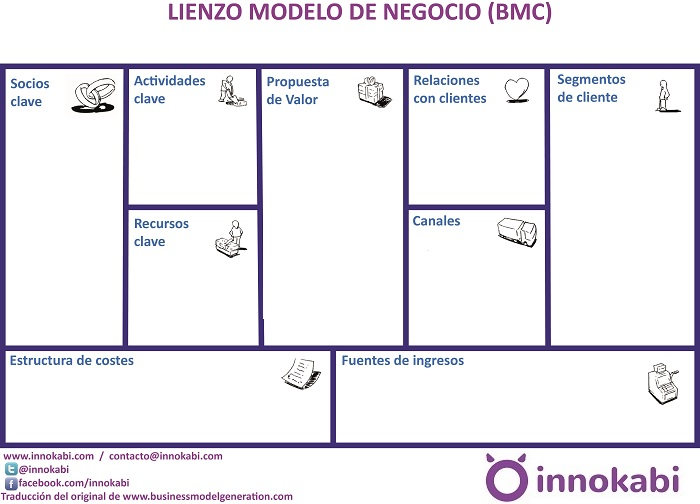
\includegraphics[width=10cm]{./Imagenes/imagen4}
\end{center}




%-----------------------------------------------------------------
\section{Ejemplo}

\par \textbf{BMC - ASECONTRI J.A.J} \\
\par La empresa ASECONTRI J.A.J se dedica a brindar
asesorías contables y tributarias a PYMES. Actualmente la empresa ofrece a sus clientes
varios productos y servicios en el área administrativa, contable y
tributaria.
\newline
\newline
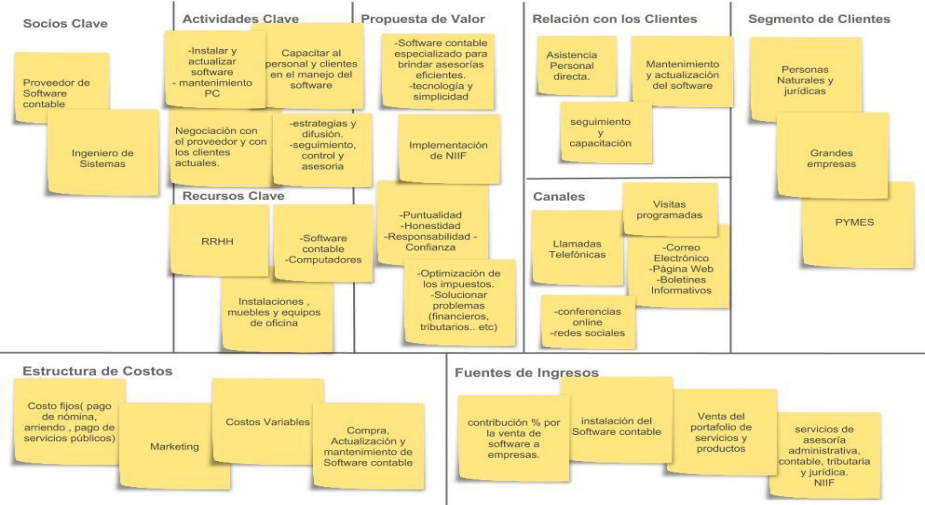
\includegraphics[width=0.55\textwidth]{./Imagenes/1}\cite{2}

\par \textbf{BSC - TRANSPORTES YAKOS SAC} 
\newline
\begin{center}
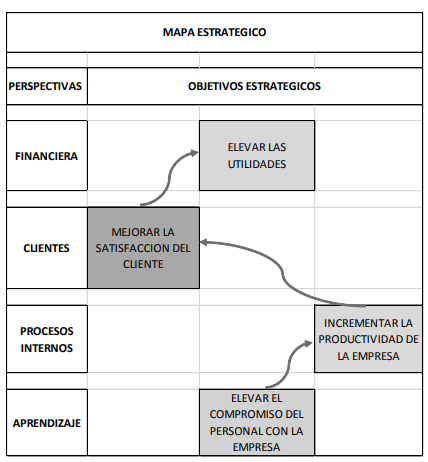
\includegraphics[width=0.45\textwidth]{./Imagenes/2}\cite{1}
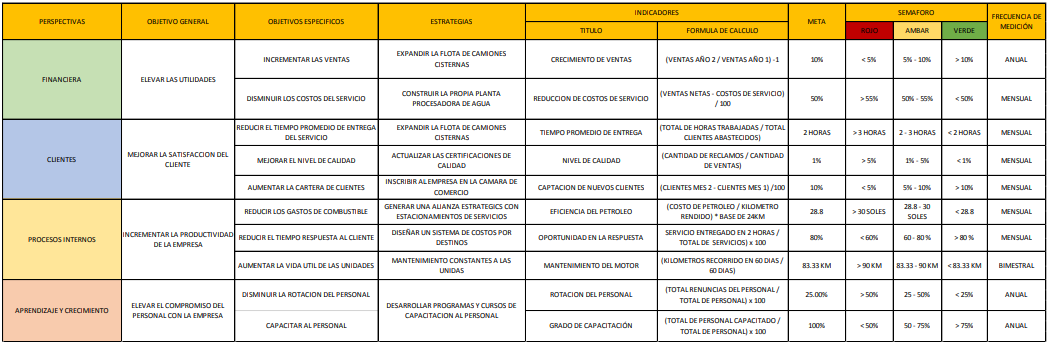
\includegraphics[width=0.5\textwidth]{./Imagenes/4} \cite{1}
\end{center}


%-----------------------------------------------------------------
\section{Análisis}

\begin{itemize}

\item  Considerar las metodologías aplicadas en este trabajo para buscar
nuevas ideas de modelo de negocio, ya que la búsqueda de la
innovación debe ser constante.
\item Asimismo, podemos generalizar que el modelo de gestión estratégica puede ser aplicable a cualquier empresa sin importar su
magnitud, ni el número de trabajadores; solo se requiere que la empresa
cuente con un plan estratégico y que quiera medir y controlar el avance de
sus objetivos.
\item El mayor problema que pueda presentarse es que una empresa defina su
plan estratégico, objetivos y estrategias ampliamente y no de acuerdo a las
cuatro perspectivas del BSC. 
\end{itemize}
%-----------------------------------------------------------------
\section{Conclusiones}

\begin{itemize}
\item El Balanced Scorecard nos ayuda a establecer y enfocar las estratégias de la empresa hacia el futuro, todo con el fin de poder convertir en realidad la visión empresarial, esto se logra a través de la suma de los objetivos de cada una de las cuatro perspectivas que nos propone mejorar el BSC.

\item Balanced Scorecard y Business model canvas son técnicas de análisis empresarial. Ambas técnicas son útiles para mejorar el desempeño organizacional. . Ambos se pueden usar junto con los indicadores clave de rendimiento para monitorear y mejorar el rendimiento de la organización. 

\end{itemize}

% Bibliografia.
%-----------------------------------------------------------------

\bibliographystyle{plain}
\bibliography{Bibliografia}

\end{document}

